\newpage
\subsection{UC4 - Modifica Grafico}
\label{subsec:uc4}

%TODO: Add correct image
\begin{figure}[h]
    \centering
    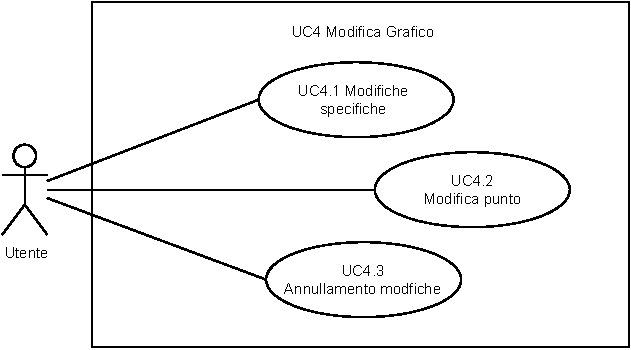
\includegraphics[width=0.8\textwidth]{componenti/casi-duso/diagrammi/UC4.pdf}
    \caption{Diagramma rappresentante UC4}
    \label{fig:UC4}
\end{figure}


\begin{itemize}
    \item \textbf{Descrizione}: L’utente modifica la visualizzazione del grafico precedentemente costruito
                                e ne vede le modifiche.
	
    \item \textbf{Attore primario}: Utente.
    
    \item \textbf{Precondizione}:   Nel programma è stato importato un dataset dotato di metatag per ogni
                                    colonna dei dati ed è stato costruito un grafico di una tipologia scelta dall'utente.

    \item \textbf{Postcondizione}:  Viene aggiornato il grafico costruito e visualizzato con i nuovi parametri.

	\item \textbf{Scenario principale}:
		\begin{enumerate}
			\item L'utente decide di modificare il grafico corrente.
			\item L'utente effettua le modifiche desiderate tra quelle rese possibili.
            \item L'utente conferma le modifiche apportate selezionando il pulsante di conferma.
        \end{enumerate}

    \item \textbf{Scenario alternativo}: % Si tratta di estensione?
        \begin{enumerate}
            \item L'utente decide di annullare le modifiche effettuate (UC4.5) al posto di confermarle.   
            \item Le modifiche vengono scartate e viene ripristinata la visualizzazione del grafico prima delle modifiche.
        \end{enumerate}
    
\end{itemize}

\newpage
\subsection{UC4.1 Modifiche specifiche}
\label{subsec:uc4.1}

%Immagine dello use case.
\begin{figure}[h]
    \centering
    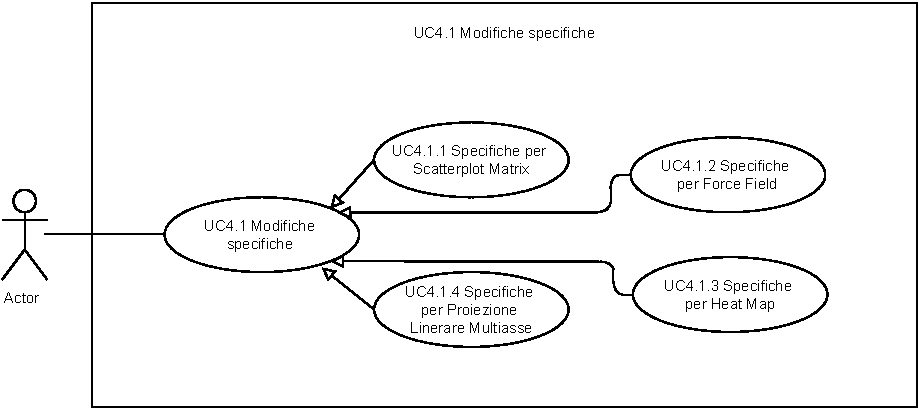
\includegraphics[width=0.8\textwidth]{componenti/casi-duso/diagrammi/UC4.1.pdf}
    \caption{Diagramma rappresentante UC4.1}
    \label{fig:UC4}
\end{figure}

%Lista che lo definisce
\begin{itemize}
    \item \textbf{Descrizione}: L’utente effettua modifica specifiche al tipo di grafico precedentemente costruito e visualizzato, 
                                su parametri quindi validi solo per tale visualizzazone, e ne vede le modifiche.
	
    \item \textbf{Attore primario}: Utente.
    
    \item \textbf{Precondizione}:   Nel programma è stato importato un dataset dotato di metatag per ogni
                                    colonna dei dati ed è stato costruito un grafico di una tipologia scelta dall'utente.

    \item \textbf{Postcondizione}:  Viene aggiornato il grafico costruito e visualizzato con i nuovi parametri.

	\item \textbf{Scenario principale}:
		\begin{enumerate}
			\item L'utente decide di modificare il grafico corrente e di modificare paraemtri specifici alla sua visualizzazione.
			\item L'utente effettua le modifiche desiderate tra quelle rese possibili.
        \end{enumerate}
    \item \textbf{Generalizzazioni}:
        \begin{itemize}
            \item Modifica Scatterplot Matrix (UC4.1.1)
            \item Modifica Force Field (UC4.1.2)
            \item Modifica Heat Map (UC4.1.3)
            \item Modifica Proiezione Lineare Multiasse (UC4.1.4)
        \end{itemize}

\end{itemize}


\newpage
\subsection{UC4.1.1 Modifica Scatterplot Matrix}
\label{subsec:uc4.1}

\begin{figure}[h]
    \centering
    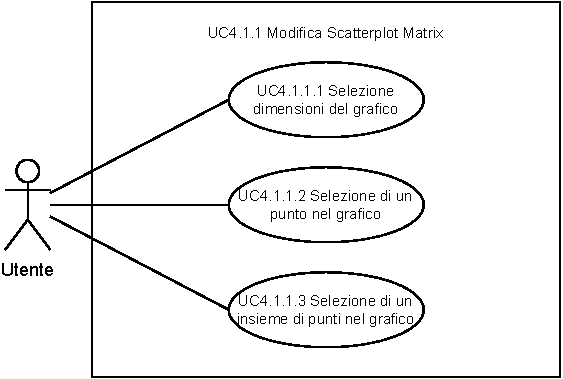
\includegraphics[width=0.6\textwidth]{componenti/casi-duso/diagrammi/UC4.1.1.pdf}
    \caption{Diagramma rappresentante UC4.1.1}
    \label{fig:UC2}
\end{figure}


\begin{itemize}
    \item \textbf{Descrizione}: L’utente modifica la visualizzazione dello Scatterplot Matrix
                                costruito dal dataset corrente.
	
    \item \textbf{Attore primario}: Utente.
    
    \item \textbf{Precondizione}:   La visualizzazione costruita dal dataset corrente è uno Scatterplot Matrix.

    \item \textbf{Postcondizione}:  Viene aggiornato il grafico costruito e visualizzato con i nuovi parametri.

	\item \textbf{Scenario principale}:
		\begin{enumerate}
            \item L'utente apporta le modifiche desiderate tra quelle offerte dallo Scatterplot Matrix.
        \end{enumerate}
\end{itemize}


\subsubsection{UC4.1.1.1 Selezione dimensioni del grafico}
\label{subsec:uc4.1.1}
\begin{itemize}
    \item \textbf{Descrizione}: L’utente dispone di dati con metadati assegnati e può 
                                scegliere fino a 5 dimensioni che possono essere  visualizzate nello Scatterplot Matrix.
	
    \item \textbf{Attore primario}: Utente.
    
    \item \textbf{Precondizione}:   La visualizzazione costruita dal dataset corrente è uno Scatterplot Matrix.
    \item \textbf{Postcondizione}:  Vengono modificate le dimensioni visualizzate nei plot dello Scatterplot Matrix.

	\item \textbf{Scenario principale}:
        \begin{enumerate}
            \item   L'utente seleziona l'opzione di selezione delle dimensioni.
            \item   L'utente seleziona fino a cinque dimensioni. 
           
            \item   Ad ogni selezione l'utente
                    sceglie una delle dimensioni attuali del grafico e la scarta.
           
            \item   La visualizzazione sostituisce le dimensioni scartate con le nuove selezionate.
        \end{enumerate}
\end{itemize}


\subsubsection{UC4.1.1.2 Selezione di un punto nel grafico}
\label{subsec:uc4.1.1}
\begin{itemize}
    \item \textbf{Descrizione}: L'utente seleziona un punto in uno Scatterplot della matrice per vedere come 
                                esso viene rappresentato negli altri grafici a dispersione della visualizzazione corrente.
	
    \item \textbf{Attore primario}: Utente.
    
    \item \textbf{Precondizione}:   La visualizzazione costruita dal dataset corrente è uno Scatterplot Matrix.
    \item \textbf{Postcondizione}:  Le proiezioni del punto selezionato, se appartentente allo Scatterplot, 
                                    venogno evidenziate in tutti i grafici della visualizzazione.

	\item \textbf{Scenario principale}:
        \begin{enumerate}
            \item L'utente seleziona un punto contente dati di uno Scatterplot della matrice.
            \item La proiezione del punto viene evidenziata in tutti gli Scatterplot della visualizzazione.
        \end{enumerate}

    \item \textbf{Scenario alternativo}:
        \begin{enumerate}
            \item L'utente seleziona un punto vuoto di uno Scatterplot della matrice.
            \item Non viene evidenziato alcun punto della matrice.
        \end{enumerate}

\end{itemize}


\subsubsection{UC4.1.1.3 Selezione di un insieme di punti del grafico}
\label{subsec:uc4.1.1}
\begin{itemize}
    \item \textbf{Descrizione}: L'utente seleziona un insieme di punti in uno Scatterplot della matrice per vedere come 
                                essi vengono rappresentati negli altri grafici a dispersione della visualizzazione corrente.
	
    \item \textbf{Attore primario}: Utente.
    
    \item \textbf{Precondizione}:   La visualizzazione costruita dal dataset corrente è uno Scatterplot Matrix.
    \item \textbf{Postcondizione}:  Le proiezioni dei punti selezionati, se appartentente allo Scatterplot, 
                                    vengono evidenziate in tutti i grafici della visualizzazione.

	\item \textbf{Scenario principale}:
        \begin{enumerate}
            \item L'utente seleziona un'aerea di punti di uno Scatterplot della matrice.
            \item Le proiezioni dei punti contenteni dati vengono evidenziati in tutti gli Scatterplot della visualizzazione.
        \end{enumerate}

    \item \textbf{Scenario alternativo}:
        \begin{enumerate}
            \item L'utente seleziona un insieme di punti vuoto.
            \item Non viene evidenziato alcun punto della matrice.
        \end{enumerate}

\end{itemize}


\newpage
\subsection{UC4.1.2 Modifica Force Field}
\label{subsec:uc4.1.2}
% TODO: Create image for force field graph.
\begin{figure}[h]
    \centering
    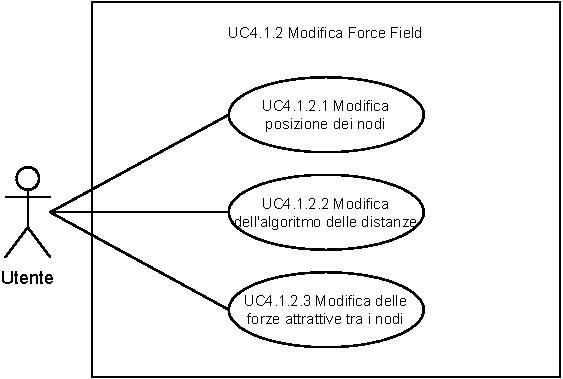
\includegraphics[width=0.6  \textwidth]{componenti/casi-duso/diagrammi/UC4.1.2.pdf}
    \caption{Diagramma rappresentante UC4.1.2}
    \label{fig:UC2}
\end{figure}


\begin{itemize}
    \item \textbf{Descrizione}: L’utente vuole modificare la visualizzazione del grafo Force Field
                                costruito dal dataset corrente.
	
    \item \textbf{Attore primario}: Utente.
    
    \item \textbf{Precondizione}:   La visualizzazione costruita dal dataset corrente è un Force Field.

    \item \textbf{Postcondizione}:  Viene aggiornato il grafico costruito e visualizzato con i nuovi parametri.

	\item \textbf{Scenario principale}:
		\begin{enumerate}
            \item L'utente apporta le modifiche desiderate tra quelle offerte dal Force Field.
        \end{enumerate}
\end{itemize}

\subsubsection{UC4.1.2.1 Modifica posizione dei nodi}
\label{subsec:uc4.1.2.1}
\begin{itemize}
    \item \textbf{Descrizione}: L’utente vuole esplorare meglio i dati e decide di 
                                modificare la posizione dei nodi del grafo, trascinandoli con il 
                                cursore nell'area definita dal grafico.
	
    \item \textbf{Attore primario}: Utente.
    
    \item \textbf{Precondizione}:   La visualizzazione costruita dal dataset corrente è un Force Field.
    \item \textbf{Postcondizione}:  Viene modificata la posizione dei nodi del grafo nella visualizzazione.

	\item \textbf{Scenario principale}:
        \begin{enumerate}
            \item L'utente tiene premuto il tasto di selezione e trascina il cursore sponstando il nodo nello spazio della visualizzazione.
            \item La visualizzazione muove i punti del grafo mantentendo le connessioni tra i nodi.
        \end{enumerate}
\end{itemize}

\subsubsection{UC4.1.2.2 Modifica dell'algoritmo delle distanze}
\label{subsec:uc4.1.2.2}
\begin{itemize}
    \item \textbf{Descrizione}: L’utente decide di cambiare l’algoritmo usato per il calcolo delle distanze.

	
    \item \textbf{Attore primario}: Utente.
    
    \item \textbf{Precondizione}:   La visualizzazione costruita dal dataset corrente è un Force Field.
    \item \textbf{Postcondizione}:  Viene modificata la distanza tra i nodi del grafo nella visualizzazione.

	\item \textbf{Scenario principale}:
        \begin{enumerate}
            \item L'utente seleziona il menu delle distanze e seleziona uno degli algoritmi presentati nel menù.
            \item La visualizzazione modifica la distanza tra i nodi secondo l'algoritmo scelto.
        \end{enumerate}
\end{itemize}

\subsubsection{UC4.1.2.3 Modifica intensità forza attrattiva tra nodi}
\label{subsec:uc4.1.2.3}
\begin{itemize}
    \item \textbf{Descrizione}: Per poter visualizzare meglio i cluster di dati l’utente 
                                decide di scalare la forza di attrattiva tra i nodi.

	
    \item \textbf{Attore primario}: Utente.
    
    \item \textbf{Precondizione}:   La visualizzazione costruita dal dataset corrente è un Force Field.
    \item \textbf{Postcondizione}:  Viene modificata l'intensità della forza attrattiva tra i nodi del grafo nella visualizzazione.

	\item \textbf{Scenario principale}:
        \begin{enumerate}
            \item L'utente seleziona la barra intensità e trascinando il cursore sulla barra varia l’intensità.
            \item La visualizzazione modifica l'intensità della forza secondo il valore selezionato nel grafo.
        \end{enumerate}
\end{itemize}


%%  _________________________
%
%%  Sezione della Heat Map
%%  _________________________
\newpage
\subsection{UC4.1.3 Modifica Heat Map}
\label{subsec:uc4.1.3}
% TODO: Create image for force field graph.
\begin{figure}[h]
    \centering
    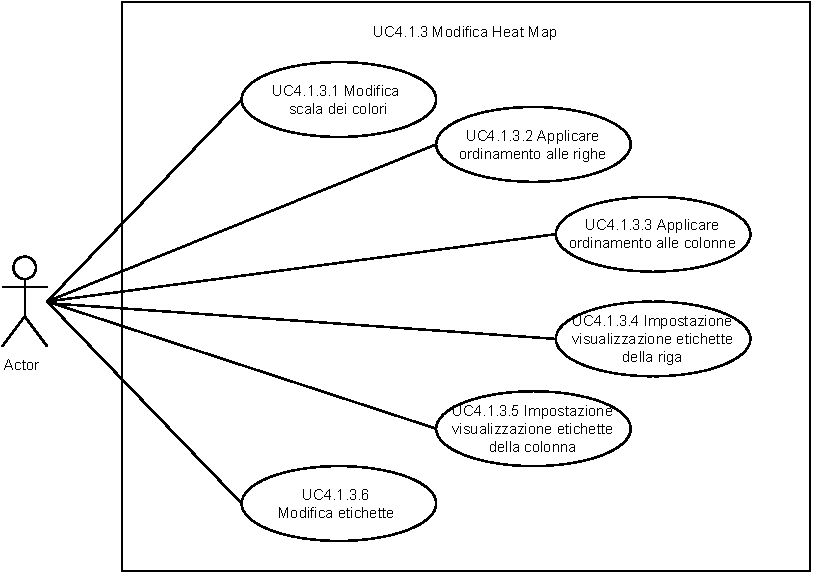
\includegraphics[width=0.6\textwidth]{componenti/casi-duso/diagrammi/UC4.1.3.pdf}
    \caption{Diagramma rappresentante UC4.1.3}
    \label{fig:UC2}
\end{figure}


\begin{itemize}
    \item \textbf{Descrizione}: L’utente vuole modificare la visualizzazione della Heat Map
                                costruita dal dataset corrente.
	
    \item \textbf{Attore primario}: Utente.
    
    \item \textbf{Precondizione}:   La visualizzazione costruita dal dataset corrente è un grafico di tipo Heat Map.

    \item \textbf{Postcondizione}:  Viene aggiornato il grafico costruito e visualizzato con i nuovi parametri.

	\item \textbf{Scenario principale}:
		\begin{enumerate}
            \item L'utente apporta le modifiche desiderate tra quelle offerte dalla Heat Map.
        \end{enumerate}
\end{itemize}

\subsubsection{UC4.1.3.1 Modifica scala dei colori}
\label{subsec:uc4.1.3.1}
\begin{itemize}
    \item \textbf{Descrizione}: L’utente vuole esplorare meglio i dati e decide di 
                                modificare la scala dei colori applicata alla Heat Map scegliendo una 
                                tra quelle proposte.
	
    \item \textbf{Attore primario}: Utente.
    
    \item \textbf{Precondizione}:   La visualizzazione costruita dal dataset corrente è una Heat Map.
    \item \textbf{Postcondizione}:  Viene modificata la scala dei colori del grafico nella visualizzazione.

	\item \textbf{Scenario principale}:
        \begin{enumerate}
            \item L'utente seleziona la voce "Scala dei colori" e seleziona una delle opzioni disponibili.
            \item La visualizzazione cambia la scala dei colori adottata dalla Heat Map.
        \end{enumerate}
\end{itemize}

\subsubsection{UC4.1.3.2 Applicare ordinamento alle righe}
\label{subsec:uc4.1.3.2}
\begin{itemize}
    \item \textbf{Descrizione}: L’utente per esplorare meglio i dati decide di ordinare le righe della Heat Map
                                seguendo l'algortimo di clustering gerarchico il quale aggiunge un dendogramma alla visualizzazione corrente.
	
    \item \textbf{Attore primario}: Utente.
    
    \item \textbf{Precondizione}:   La visualizzazione costruita dal dataset corrente è una Heat Map.
    \item \textbf{Postcondizione}:  Le righe della Heat Map vengono visualizzati secondo l'ordine imposto dall'algoritmo di ordinamento.

	\item \textbf{Scenario principale}:
        \begin{enumerate}
            \item   L'utente seleziona la casella di ordinamento delle righe.
            \item   La visualizzazione aggiorna l'ordinamento delle righe della Heat Map e viene aggiunto 
                    il dendogramma relativo alle righe.
        \end{enumerate}
\end{itemize}

\subsubsection{UC4.1.3.3 Applicare ordinamento alle colonne}
\label{subsec:uc4.1.3.3}
\begin{itemize}
    \item \textbf{Descrizione}: L’utente per esplorare meglio i dati decide di ordinare le colonne della Heat Map
                                seguendo l'algortimo di clustering gerarchico il quale aggiunge un dendogramma alla visualizzazione corrente.
	
    \item \textbf{Attore primario}: Utente.
    
    \item \textbf{Precondizione}:   La visualizzazione costruita dal dataset corrente è una Heat Map..
    \item \textbf{Postcondizione}:  Le colonne della Heat Map vengono visualizzati secondo l'ordine imposto dall'algoritmo di ordinamento.

	\item \textbf{Scenario principale}:
        \begin{enumerate}
            \item   L'utente seleziona la casella di ordinamento delle colonne.
            \item   La visualizzazione aggiorna l'ordinamento delle colonne della Heat Map 
                    e viene aggiunto il dendogramma relativo alle righe.
        \end{enumerate}
\end{itemize}


\subsubsection{UC4.1.3.4 Impostazione etichette righe}
\label{subsec:uc4.1.3.4}
\begin{itemize}
    \item \textbf{Descrizione}: L’utente decide se visualizzare le etichette relative alle righe della Heat Map.

    \item \textbf{Attore primario}: Utente.
    
    \item \textbf{Precondizione}:   La visualizzazione costruita dal dataset corrente è una Heat Map.
    \item \textbf{Postcondizione}:  La visualizzazione della Heat Map mostra le etichette delle righe se così scelto dall'utente.

	\item \textbf{Scenario principale}:
        \begin{enumerate}
            \item   L'utente seleziona se visualizzare le etichette per le righe della Heat Map.
            \item   La visualizzazione aggiorna la visibilità delle etichette delle righe in base alla selezione dell'utente.
                    
        \end{enumerate}
\end{itemize}



\subsubsection{UC4.1.3.5 Impostazione etichette colonne}
\label{subsec:uc4.1.3.5}
\begin{itemize}
    \item \textbf{Descrizione}: L’utente decide se visualizzare le etichette relative alle colonne della Heat Map.

    \item \textbf{Attore primario}: Utente.
    
    \item \textbf{Precondizione}:   La visualizzazione costruita dal dataset corrente è una Heat Map.
    \item \textbf{Postcondizione}:  La visualizzazione della Heat Map mostra le etichette delle colonne se così scelto dall'utente.

	\item \textbf{Scenario principale}:
        \begin{enumerate}
            \item   L'utente seleziona se visualizzare le etichette per le colonne della Heat Map.
            \item   La visualizzazione aggiorna la visibilità delle etichette delle colonne in base alla selezione dell'utente.
                    
        \end{enumerate}
\end{itemize}


\subsubsection{UC4.1.3.6 Modifica etichette}
\label{subsec:uc4.1.3.6}
\begin{itemize}
    \item \textbf{Descrizione}: L’utente decide di modificare una o più etichette associate alla Heat Map.

    \item \textbf{Attore primario}: Utente.
    
    \item \textbf{Precondizione}:   La visualizzazione costruita dal dataset corrente è una Heat Map.
    \item \textbf{Postcondizione}:  Le etichette della Heat Map vengono aggiornate se modificate.
	\item \textbf{Scenario principale}:
        \begin{enumerate}
            \item   L'utente seleziona le etichette da modificare e le modifica.
            \item   La visualizzazione aggiorna le etichette della Heat Map. %todo: rimuovo? 
        \end{enumerate}
\end{itemize}



\newpage
\subsection{UC4.1.4 Modifica Proiezione Lineare Multiasse}
\label{subsec:uc4.1.4}
% TODO: Create image for force field graph.
\begin{figure}[h]
    \centering
    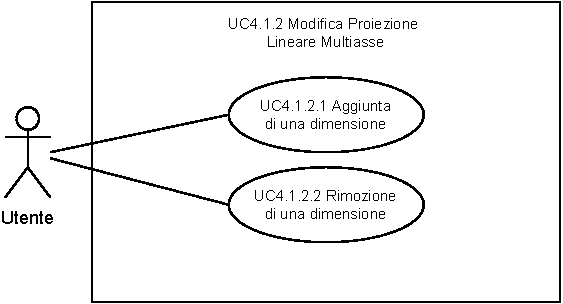
\includegraphics[width=0.8\textwidth]{componenti/casi-duso/diagrammi/UC4.1.4.pdf}
    \caption{Diagramma rappresentante UC4.1.4}
    \label{fig:UC4.1.4}
\end{figure}


\begin{itemize}
    \item \textbf{Descrizione}: L’utente vuole modificare la visualizzazione della Proiezione Lineare Multiasse
                                costruita dal dataset corrente.
	
    \item \textbf{Attore primario}: Utente.
    
    \item \textbf{Precondizione}:   La visualizzazione costruita dal dataset corrente è un grafico di tipo Proiezione Lineare Multiasse.
    \item \textbf{Postcondizione}:  Viene aggiornato il grafico costruito e visualizzato con i nuovi parametri.

	\item \textbf{Scenario principale}:
		\begin{enumerate}
            \item L'utente apporta le modifiche desiderate tra quelle offerte dalla Proiezione Lineare Multiasse.
        \end{enumerate}
\end{itemize}

\subsubsection{UC4.1.4.1 Aggiunta di una dimensione}
\label{subsec:uc4.1.4.1}
\begin{itemize}
    \item \textbf{Descrizione}: L’utente decide di visualizzare maggiori informazioni
                                aggiungendo una dimensione al grafico.

    \item \textbf{Attore primario}: Utente.
    
    \item \textbf{Precondizione}:   La visualizzazione costruita dal dataset corrente è una Proiezione Lineare Multiasse.
    \item \textbf{Postcondizione}:  La visualizzazione della PLA aggiunge una dimenisone.

	\item \textbf{Scenario principale}:
        \begin{enumerate}
            \item L'utente seleziona la voce "Dimensioni" e seleziona una dimensione da aggiungere alla proiezione.
            \item La visualizzazione aggiugne la dimensione selezionata e riposiziona i punti.
           
        \end{enumerate}
\end{itemize}

\subsubsection{UC4.1.4.2 Rimozione di una dimensione}
\label{subsec:uc4.1.4.2}
\begin{itemize}
    \item \textbf{Descrizione}: L’utente decide di rimuovere una dimensione dalla Proiezione Lineare Multiasse
                                a patto che essa non sia monodimensionale.

    \item \textbf{Attore primario}: Utente.
    
    \item \textbf{Precondizione}:   La visualizzazione costruita dal dataset corrente è una Proiezione Lineare Multiasse
                                    e rappresenta almeno due dimensioni.
    \item \textbf{Postcondizione}:  La visualizzazione della PLA rimuove una dimenisone.

	\item \textbf{Scenario principale}:
        \begin{enumerate}
            \item L'utente seleziona la voce "Dimensioni" e seleziona una dimensione da rimuovere dalla proiezione.
            \item La visualizzazione rimuove la dimensione selezionata e riposiziona i punti.
           
        \end{enumerate}
\end{itemize}


\newpage

\begin{figure}[h]
    \centering
    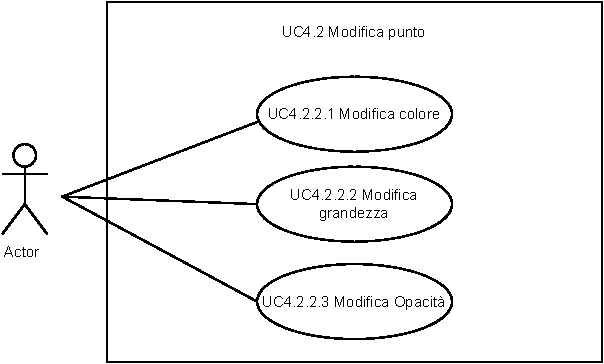
\includegraphics[width=0.8\textwidth]{componenti/casi-duso/diagrammi/UC4.2.pdf}
    \caption{Diagramma rappresentante UC4.2}
    \label{fig:UC4.2}
\end{figure}


\subsection{UC4.2 Modifica proprietà punti di una dimensione}
\label{subsec:uc4.2}
\begin{itemize}
    \item \textbf{Descrizione}: L’utente decide di manipolare la rappresentazione dei punti del grafico.
	
    \item \textbf{Attore primario}: Utente.
    
    \item \textbf{Precondizione}:   La visualizzazione costruita dal dataset corrente non è una Heat Map.

    \item \textbf{Postcondizione}:  Viene modificato lo stile dei punti per una determinata dimensione della visualizzazione.

	\item \textbf{Scenario principale}:
        \begin{enumerate}
        
            \item L'utente seleziona il menu delle dimensioni e ne sceglie una.
            \item L'utente manipola le proprietà che gli interessano.
            \item La visualizzazione mostra i nuovi punti per la dimensione selezionata.
                
        \end{enumerate}
\end{itemize}


\subsubsection{UC4.2.1 Modifica colore}
\label{subsec:uc4.2.1}
\begin{itemize}
    \item \textbf{Descrizione}: L'utente decide di modificare il colore di nodi relativi ad una dimensione.

	
    \item \textbf{Attore primario}: Utente.
    
    \item \textbf{Precondizione}:   L'utente ha selezionato l'opzione di modifica delle proprietà dei nodi per dimensione (UC4.2.4).
    \item \textbf{Postcondizione}:  Viene aggiornato il colore dei nodi della dimensione selezionata.

	\item \textbf{Scenario principale}:
        \begin{enumerate}
            \item L'utente seleziona il nuovo colore da assegnare ai nodi tra quelli resi disponbili.
        \end{enumerate}
\end{itemize}

\subsubsection{UC4.2.2 Modifica raggio}
\label{subsec:uc4.2.2}
\begin{itemize}
    \item \textbf{Descrizione}: L'utente decide di modificare il raggio di nodi relativi ad una dimensione.
	
    \item \textbf{Attore primario}: Utente.
    
    \item \textbf{Precondizione}:   L'utente ha selezionato l'opzione di modifica delle proprietà dei nodi per dimensione (UC4.2.4).
    \item \textbf{Postcondizione}:  Viene aggiornato il raggio dei nodi della dimensione selezionata.

	\item \textbf{Scenario principale}:
        \begin{enumerate}
            \item L'utente fa variare il raggio dei nodi mediante uno slider.
        \end{enumerate}
\end{itemize}

\subsubsection{UC4.2.3 Modifica opacità}
\label{subsec:uc4.2.3}
\begin{itemize}
    \item \textbf{Descrizione}:  L'utente decide di modificare l'opacità dei nodi relativi ad una dimensione.

	
    \item \textbf{Attore primario}: Utente.

    \item \textbf{Precondizione}: L'utente ha selezionato l'opzione di modifica delle proprietà dei nodi per dimensione (UC4.2.4).
    \item \textbf{Postcondizione}:  Viene aggiornata l'opacità dei nodi della dimensione selezionata.

	\item \textbf{Scenario principale}:
        \begin{enumerate}
            \item L'utente fa variare l'opacità dei nodi mediante uno slider.
        \end{enumerate}
\end{itemize}


\subsection{UC4.3 Annulamento delle modifiche}

\begin{itemize}
    \item \textbf{Descrizione}: L'utente decide di scartare le modifiche fatte nella corrente selezione di modifica.

    \item \textbf{Attore primario}: Utente.
    
    \item \textbf{Precondizione}:   L'utente ha selezionato la voce di Modifica Grafico dal menu.
    \item \textbf{Postcondizione}:  Viene ripristinato il grafo ai parametri precedenti della selezione e visualizzato.

	\item \textbf{Scenario principale}:
        \begin{enumerate}

            \item L'utente seleziona il pulsante "Annulla modifiche".
            \item HDviz ripristina i parametri del grafo ai valori precedenti alla selezione del menu di modifica.
        
        \end{enumerate}
\end{itemize}



